\addcontentsline{toc}{chapter}{Messdaten}
\label{Protokoll}

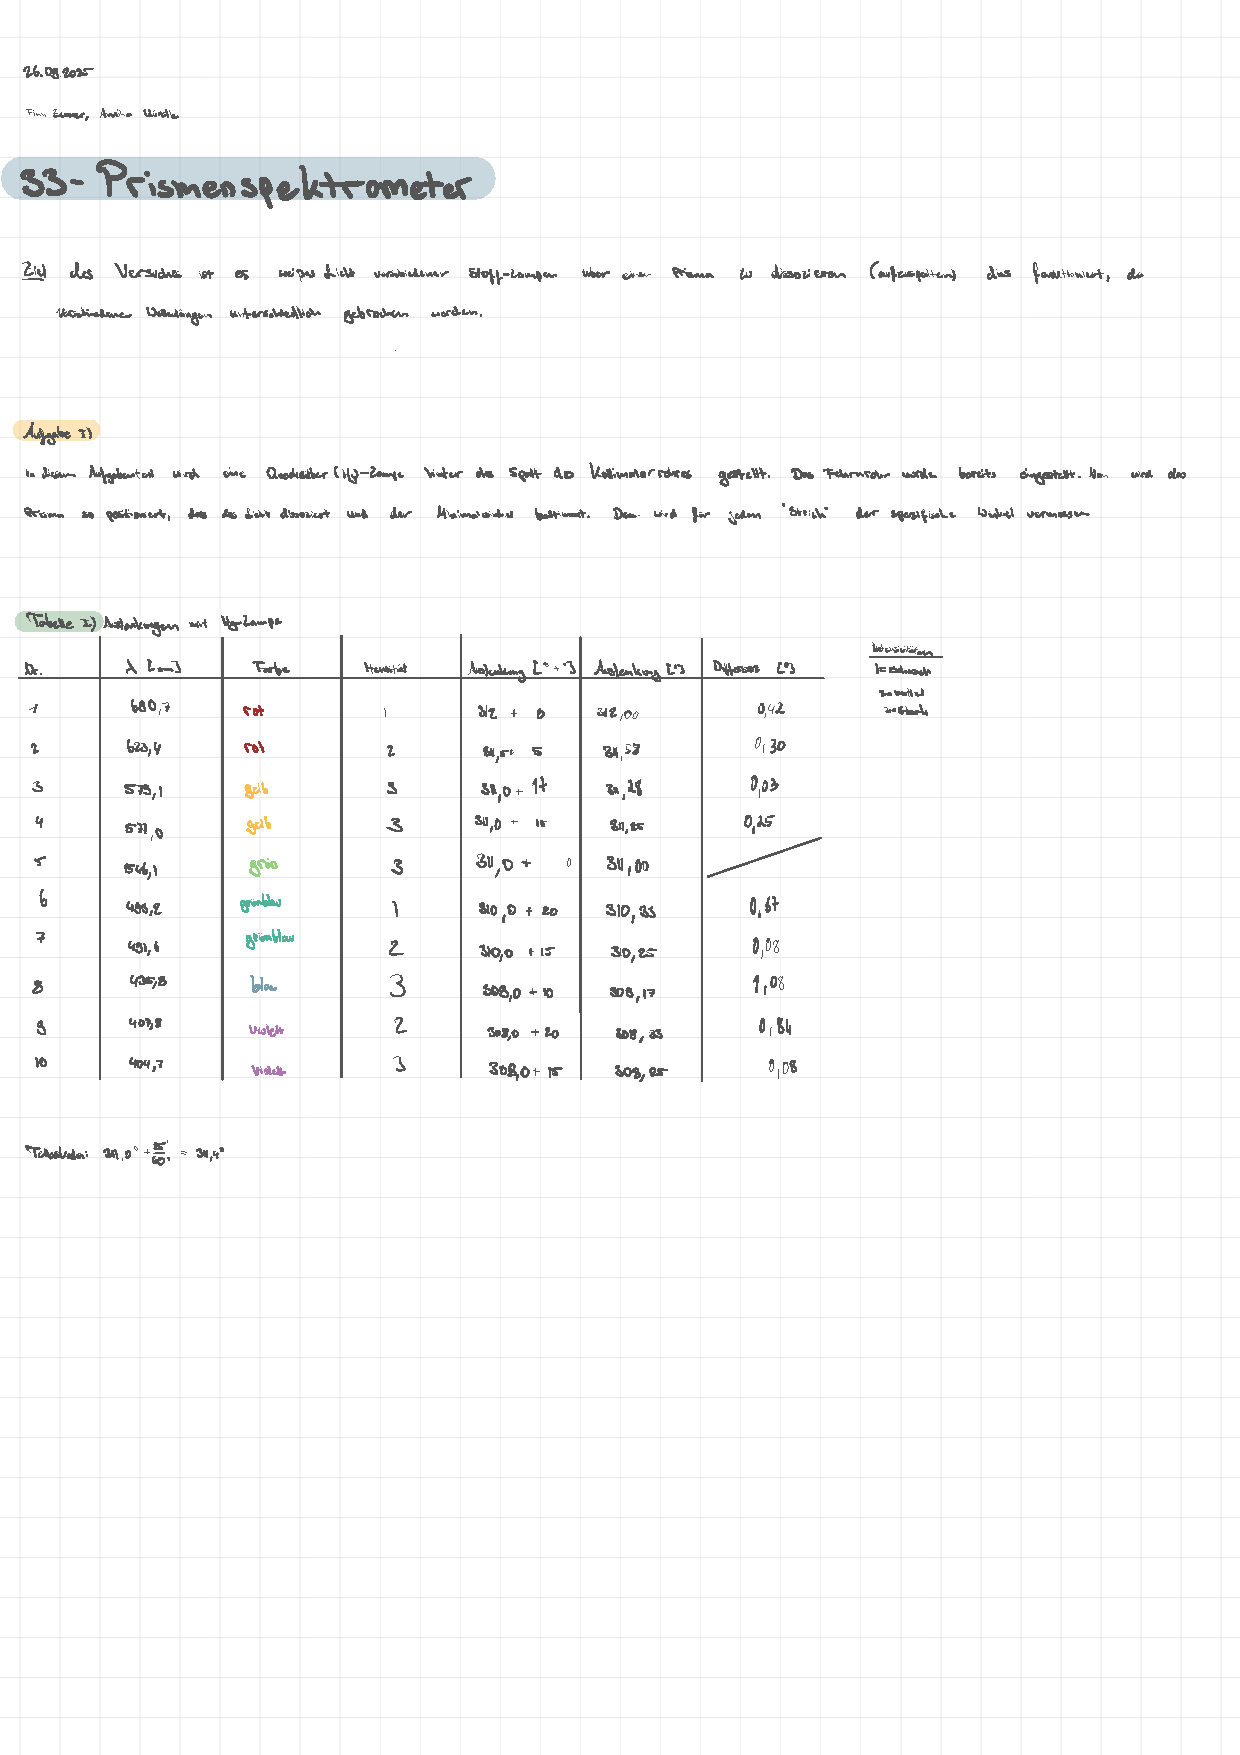
\includepdf[
  pages=1-2,               
  pagecommand={\thispagestyle{empty}} 
]{Protokolle/\versuchsnummer/Chapter/Messprotokoll.pdf}

\begin{figure}
  \centering
  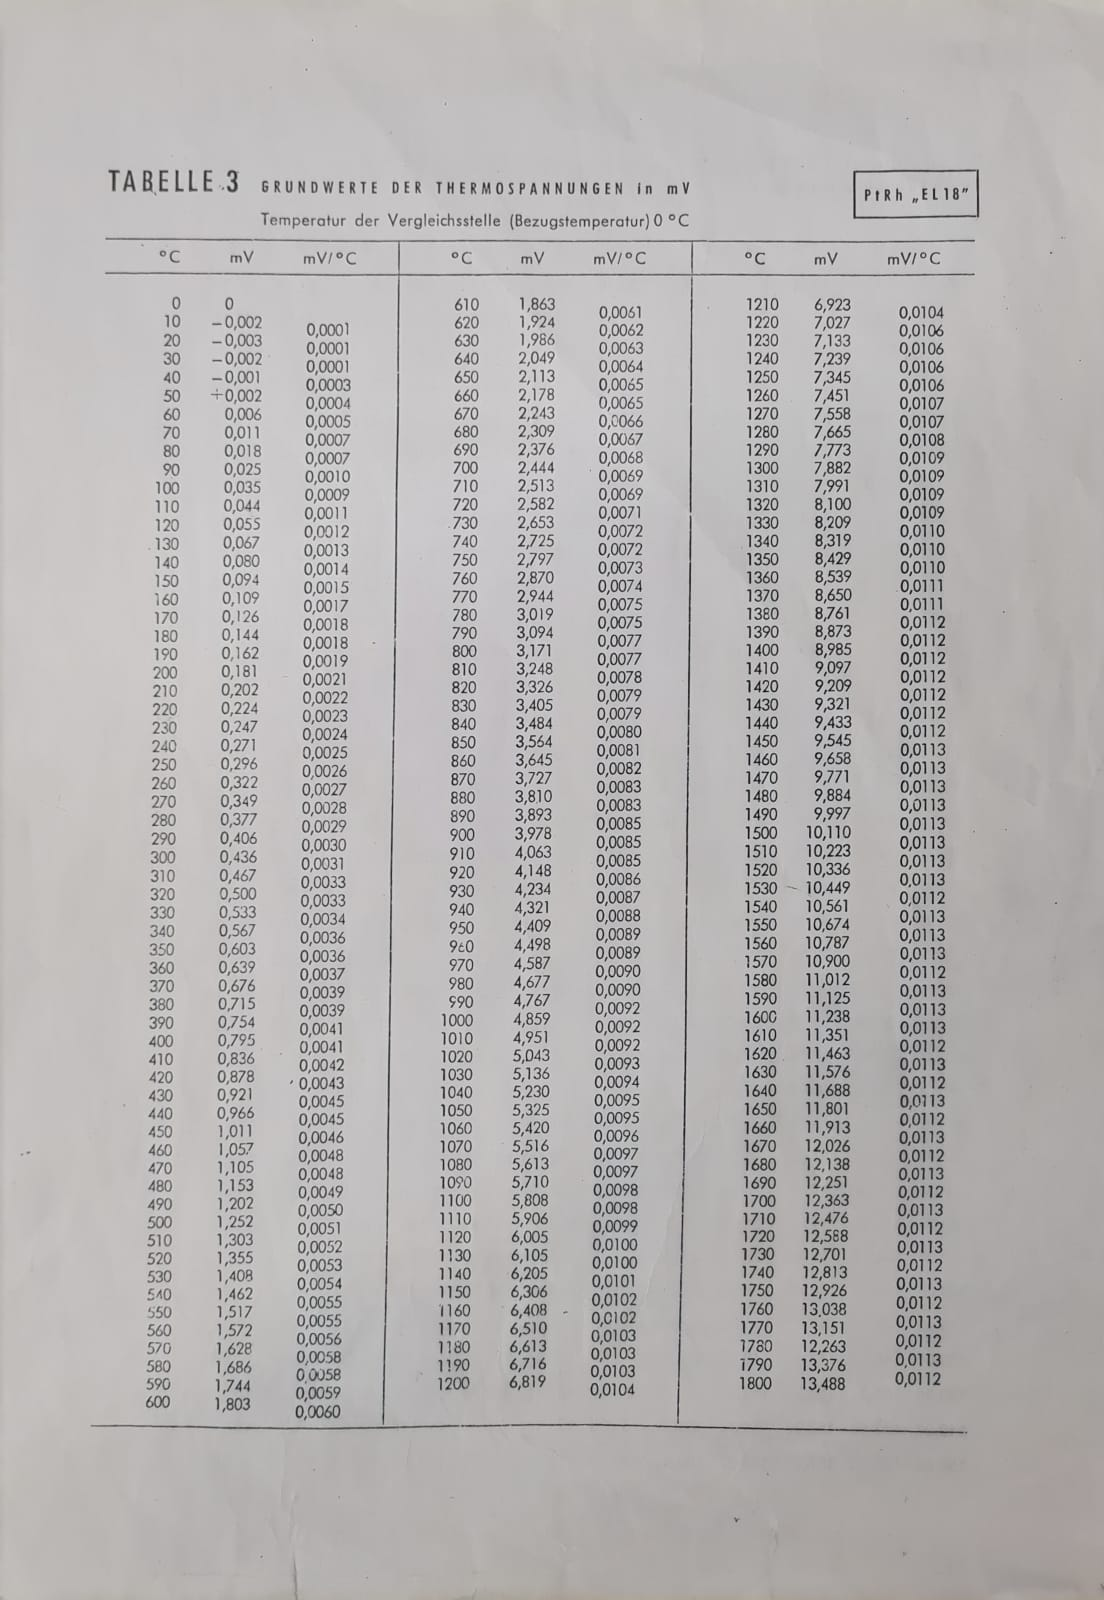
\includegraphics[width=\textwidth]{img/41/tabelle.jpg}
\end{figure}


\addcontentsline{lot}{table}{\protect\numberline{\thechapter.1} Vergleich Zwei- und Vierleiter}
% \addcontentsline{lot}{table}{\protect\numberline{\thechapter.2} Trägheitsmoment der regelmäßigen Messingplatte}
% \addcontentsline{lot}{table}{\protect\numberline{\thechapter.3} Trägheitsmoment der unregelmäßigen Messingplatte}
% \addcontentsline{lot}{table}{\protect\numberline{\thechapter.4} Schtein'scher Satz}
